\documentclass[a4paper,12pt]{article}
\usepackage[T1]{fontenc}
\usepackage[utf8]{inputenc}
\usepackage{graphicx}
\usepackage{amsmath}
\usepackage{amsfonts}
\usepackage{amssymb}
\usepackage{booktabs}
\usepackage{float}
\usepackage{geometry}
\usepackage[german]{babel}
\usepackage{enumitem}
\usepackage{parskip}
\usepackage{underscore}
\usepackage{hyperref}
\usepackage{icomma}
% \usepackage{multicol}

\geometry{a4paper, left=25mm, right=25mm, top=20mm, bottom=20mm}

%%%%%%%%%%%%%%% Titelblatt %%%%%%%%%%%%%%%
\begin{document}
\begin{titlepage}
    \centering
    
\includegraphics[scale = 0.03]{bilder/JKU_Logo.png}\\[1.0 cm]	% JKU Logo
    \textsc{\Large Einführungspraktikum Physik}\\[0.5 cm]	        % LVA Name
    \textsc{\large 3. Versuch}\\[0.5 cm]				            % Versuch Nummer    // [x] TODO: Versuch Nummer anpassen
    \rule{\linewidth}{0.4 mm} \\[0.4 cm]
    { \huge \bfseries Brennweite}\\                                 % Versuch Name      // [x] TODO: Versuch Name anpassen
    \rule{\linewidth}{0.4 mm} \\[1.5 cm]
    \begin{minipage}{0.8\textwidth}
        \begin{flushleft} \large
            \emph{Autoren:}\\
            Eva Brandstätter (k12406599)\\
            Tobias Mittermair (k12412801)\\
            \vspace{1cm}
            \emph{Gruppe:}\\
            Freitag Vormittag\\
            \vspace{1cm}
            \emph{Betreuer:}\\
            Gerald Gmachmeir
        \end{flushleft}
        \begin{flushright} \large
            \vspace{8cm}
            \emph{Abgabe:} \\
            \today
        \end{flushright}
    \end{minipage}~    
\end{titlepage}

%%%%%%%%%%%%%%% Inhaltsverzeichnis %%%%%%%%%%%%%%%
\tableofcontents
\newpage


%%%%%%%%%%%%%%% Inhalt %%%%%%%%%%%%%%%
\section{Einleitung}
%//[ ] TODO: Einleitung
% Was soll gemessen werden? (Ziel / Motivation / Hypothese / erwartetes Ergebnis)

In diesem Versuch soll die Brennweite und die zugehörige Unsicherheit einer Sammellinse durch 
das Bessel-Verfahren bestimmt werden.

\section{Grundlagen}
%//[ ] TODO: Grundlagen
% (kurz!) Was muss ich über die zu messende Größe wissen?

% Größe s beschreiben (Bezug auf optische bank)

Das Bessel-Verfahren leitet sich aus der Annäherung an achsennahe Parallelstrahlen und einer dünnen Sammellinse ab.
Diese Umstände sind annähernd erfüllt.
Der genaue Ablauf des Verfahrens kann der Versuchsdurchführung \ref{sec:Durchfuehrung} entnommen werden.

Die Formel zur Berechnung der Brennweite $f$ mit dem Bessel-Verfahren lautet:

\begin{equation}
    \label{eq:BesselBrennweite}
    f = \frac{s^2 - e^2}{4s}
\end{equation}

wobei $s$ der Abstand zwischen Gegenstand und Schirm und $e$ der Abstand zwischen den beiden
Positionen ($e_1$, $e_2$), an denen das Bild scharf ist, ist. Die Positionen $e_1$ und $e_2$
sind dabei symmetrisch zum Mittelpunkt von $s$.

Damit es tatsächlich zwei Positionen gibt, an denen ein scharfes Bild entsteht, muss der Gegenstand
in beiden Positionen weiter als $f$ von der Linse entfernt sein. Daraus folgt die Bedingung $s>4f$.

Als Anhaltspunkt für die Brennweite wird eine zweite Methode angewandt, die ein schnelles,
aber ungenaues Ergebnis liefert: es wird ausgenutzt, dass sich Parallelstrahlen annähernd in einem Punkt schneiden, wenn sie durch eine
Sammellinse fokussiert werden. Dieser Punkt ist der Brennpunkt der Linse und befindet sich in der Entfernung $f$
von der Linse.

\begin{equation}
    \label{eq:BesselAbstand}
    e = e_2 - e_1
\end{equation}

Da bei der Ermittlung der Position der Linse für eine Scharfstellung die Schärfe nur schwer (und nur subjektiv)
beurteilt werden kann, wird je ein Intervall $[e_{i_\mathrm{links}};e_{i_\mathrm{rechts}}]$ für $e_1$ und
$e_2$ bestimmt, in dem das Bild gerade noch scharf ist. Daraus wird $e_i$ folgendermaßen berechnet.

\begin{equation}
    \label{eq:BesselAbstandIntervall}
    e_i = \frac{e_{i_\mathrm{rechts}} + e_{i_\mathrm{links}}}{2}
\end{equation}

Da die Größen $s$, $e_{i_\mathrm{rechts}}$ und $e_{i_\mathrm{links}}$ gemessen wurden, sind sie mit einer
Messunsicherheit behaftet, deshalb wird die (Gauß'sche) Fortpflanzung von Unsicherheiten angewendet,
um daraus die Unsicherheit der Brennweite $u_f$ zu berechnen. Diese lautet wie folgt:

\begin{equation}
    \label{eq:GaussUnsFortpfl}
    u_f = \sqrt{\left(\frac{\partial f}{\partial s}\right)^2 \cdot u_s^2 + \left(\frac{\partial f}{\partial e}\right)^2 \cdot u_e^2}
\end{equation}

die partiellen Ableitungen lauten:

\begin{equation}
    \frac{\partial f}{\partial s} = \frac{s^2+e^2}{4s^2}
\end{equation}

\begin{equation}
    \frac{\partial f}{\partial e} = -\frac{e}{2s}
\end{equation}

daraus ergibt sich eingesetzt in die Gleichung \ref{eq:GaussUnsFortpfl}

\begin{equation}
    \label{eq:BesselBrennwUnsFortpfl}
    u_f(s,e) = \sqrt{\left(\frac{s^2+e^2}{4s^2}\right)^2 \cdot u_s^2 + \left(-\frac{e}{2s}\right)^2 \cdot u_e^2}
\end{equation}

Nun können die, aus den verschiedenen $s_i$ ermittelten, $f_i$ per gewichtetem Mittelwert zu einem
mittleren $\bar{f_g}$ zusammengefasst werden. Die Gewichte $g_i$ entsprechen dabei den inversen
Varianzen.

\begin{equation}
    \label{eq:Gewicht}
    g_i = \frac{1}{u_{f_i}^2}
\end{equation}

\begin{equation}
    \label{eq:Mittelwert}
    \bar{f_g} = \frac{\sum_{i=1}^{N} g_i \cdot f_i}{\sum_{i=1}^{N} g_i}
\end{equation}

Dieser gewichtete Mittelwert verfügt auch über eine gewichtete Unsicherheit $u_{\bar{f_g}}$.

\begin{equation}
    \label{eq:GewichtUnsicherheit}
    u_{\bar{f_g}} = \sqrt{\frac{1}{\sum_{i=1}^{N} g_i}}
\end{equation}

\section{Versuchsbeschreibung}
\subsection{Versuchsaufbau}
%//[x] TODO: Versuchsaufbau
% Wie sieht der Versuchsaufbau aus? (Skizze, Anleitung, Geräte, …)
% auf Abbildungen Bezug nehmen

Der Versuch wurde am 13.12.2024 im Praktikumsraum P122 an der JKU in Linz zwischen 11:15 und
13:15 durchgeführt.

Für diesen Versuch wurden eine Sammellinse, ein Lineal, eine optische Bank (mit Reitern, LED
mit Kondensorlinse, Geodreieck als Objekt und Schirm) bereitgestellt.
Weiters stand ein Laptop zur Führung des Laborprotokolls und zur Dokumentation der Werte bereit.
In der nachstehenden Abbildung \ref{Abb:Versuchsaufbau1} ist der Aufbau des Versuches dargestellt.
Dabei ist zu erkennen, dass von links weg eine LED mit Kondensorlinse, danach der Objektträger
mit Geodreieck und darauffolgend eine Linse, vor dem sich ganz rechts befindenden Schirm auf der
optischen Bank angeordnet sind.

% Bild vom Versuchsaufbau
\begin{figure}[H]
    \centering
    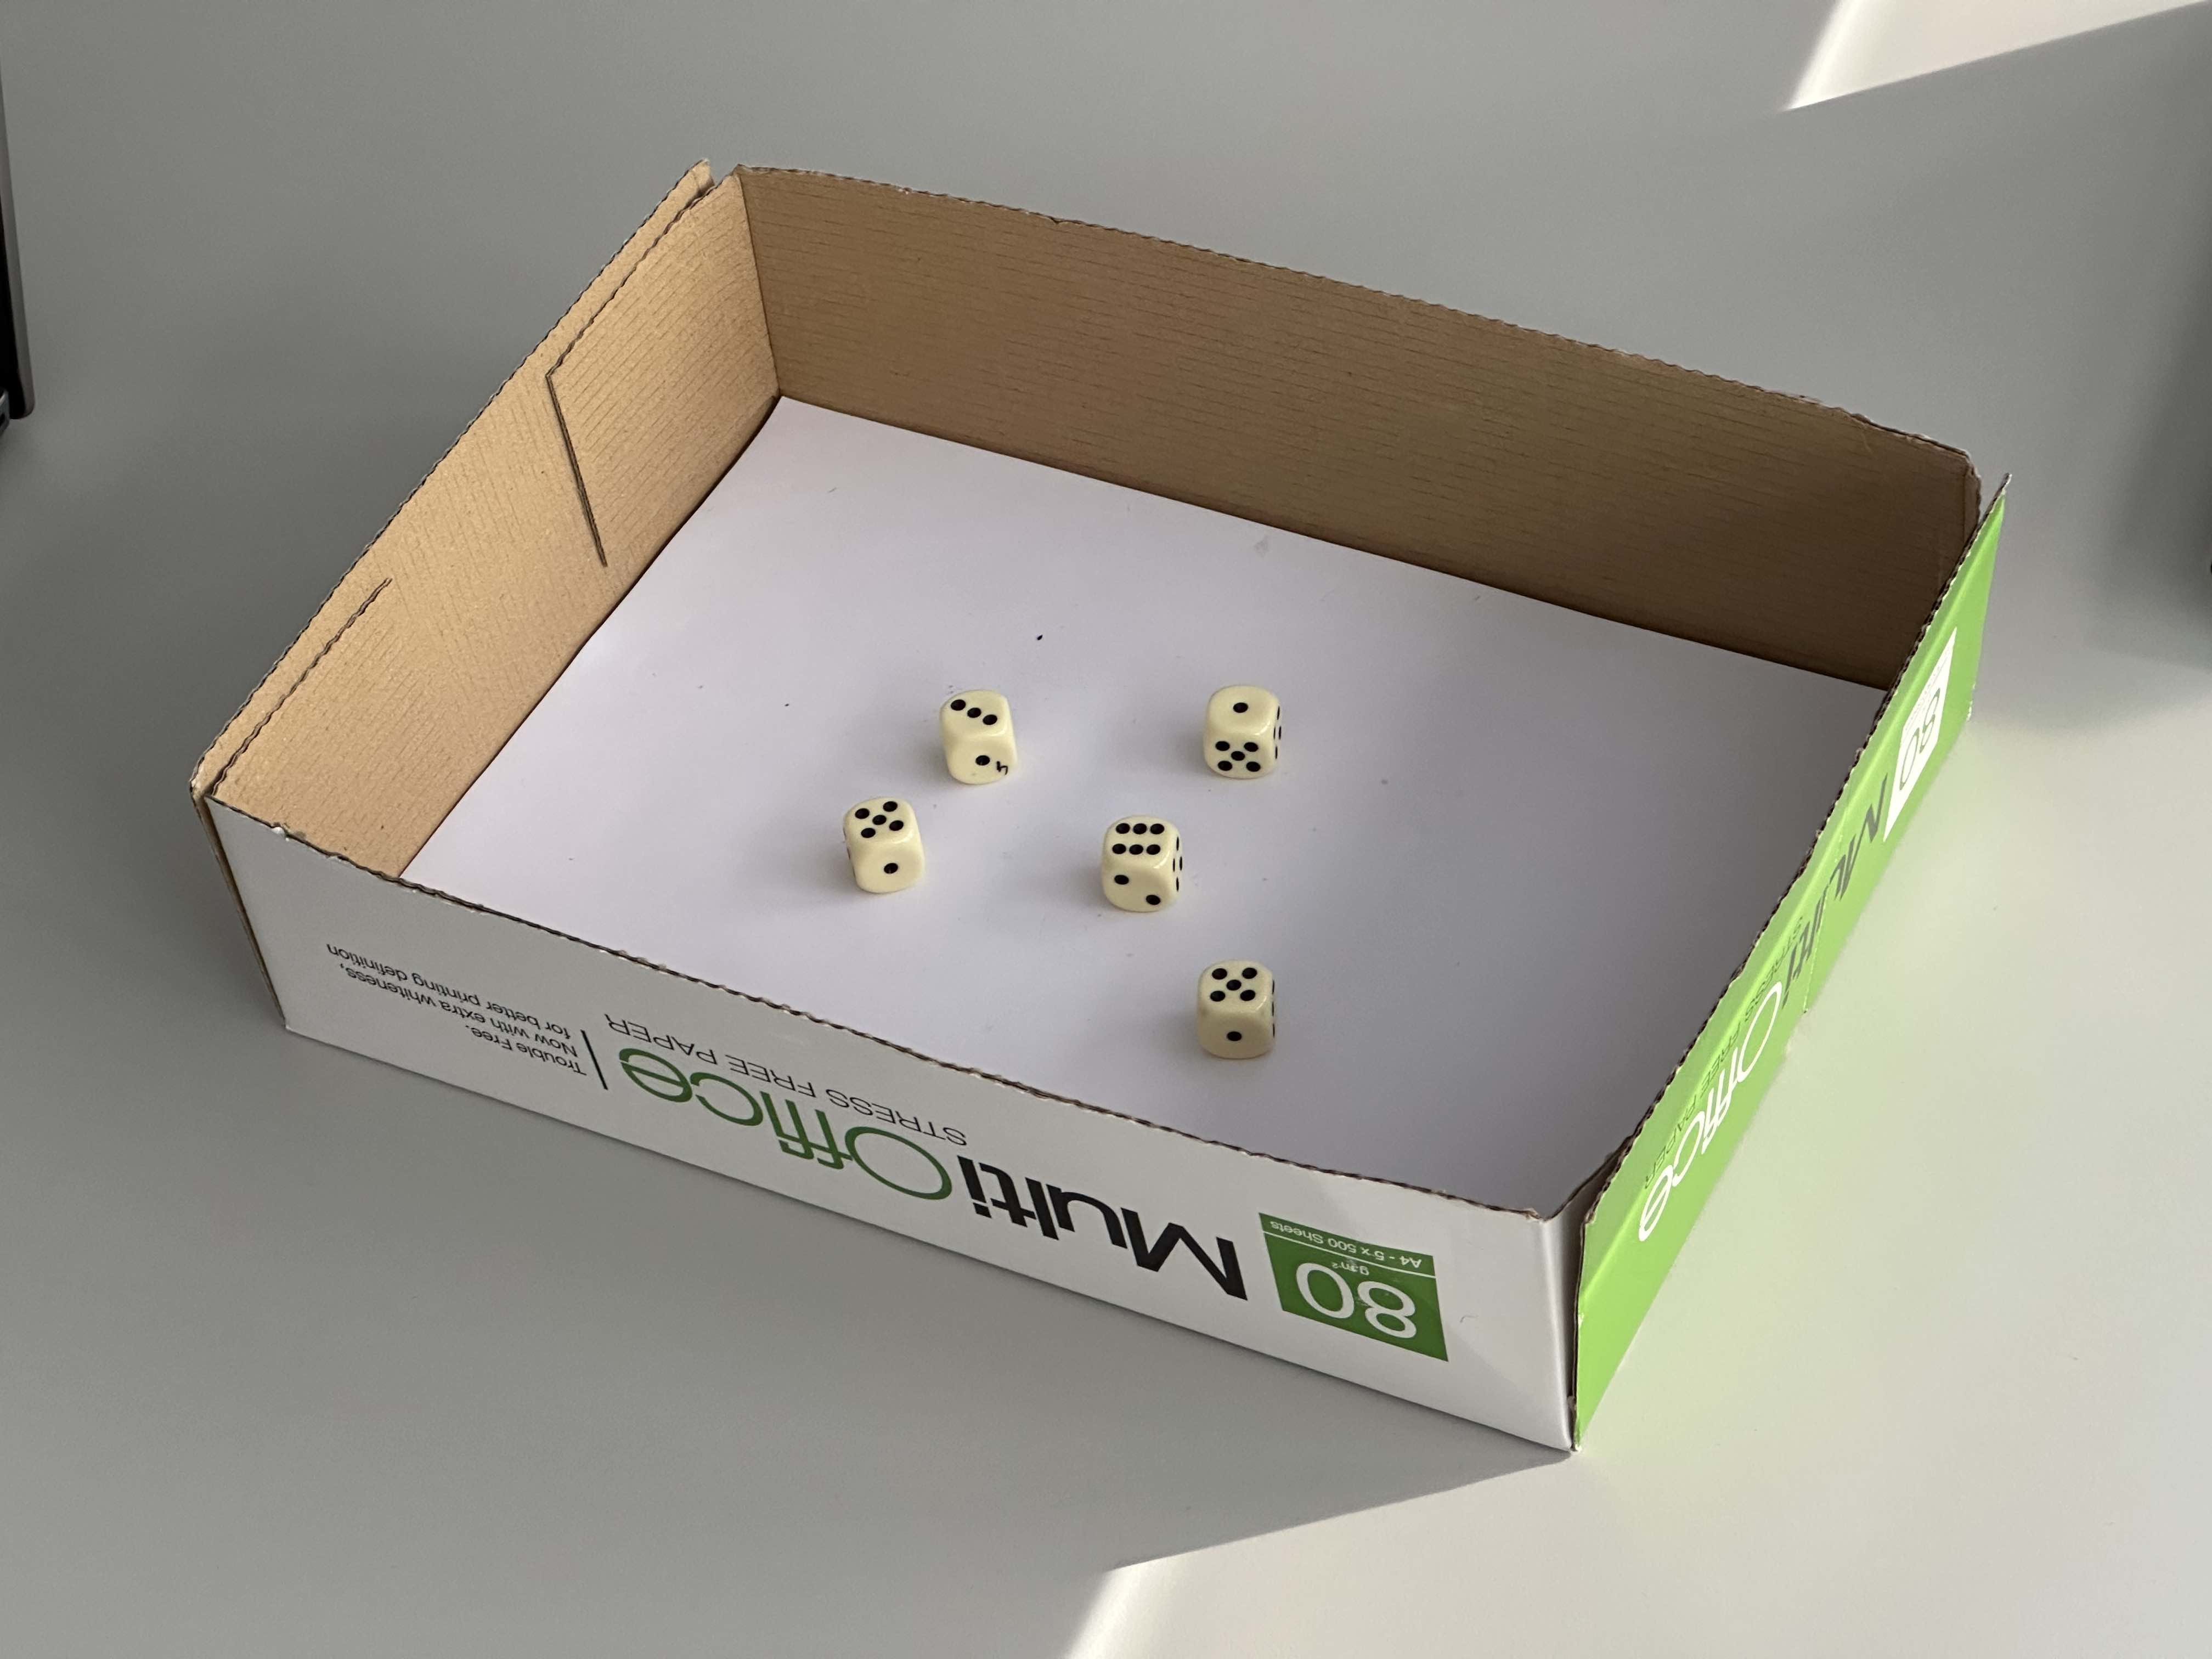
\includegraphics[width=0.5\textwidth]{bilder/Versuchsaufbau1.jpg}           %// [x] TODO: Versuchsaufbau Bild anpassen
    \caption{optische Bank mit optischen Elementen}                             %// [x] TODO: Versuchsaufbau Bildunterschrift anpassen
    \label{Abb:Versuchsaufbau1}
\end{figure}

\subsection{Durchführung}
\label{sec:Durchfuehrung}
%//[ ] TODO: Durchführung
% Wie wurde der Versuch durchgeführt bzw. ausgewertet?
% auch wann und wo?

Vor dem tatsächlichen Versuch wurde zuerst die Brennweite der Linse grob abgeschätzt.
Dabei wurde die Linse über den Labortisch gehalten und so lange auf und ab bewegt, bis das
Abbild der Deckenbeleuchtung scharf erkennbar war. Der Abstand zwischen Linse und Abbildung
wurde dann mit dem Lineal abgemessen. Dieser Abstand entspricht annähernd der Brennweite
der Linse und beträgt ungefähr 9,6cm $\pm\:1\mathrm{cm}$. Dies kann man sagen, da der Abstand
zur Deckenleuchte im Verhältnis zum Abstand der Abbildung zur Linse hinreichend groß ist.

Nun kann mit dem eigentlichen Versuch begonnen werden, da jetzt $s>4f$ gewählt werden kann.
Nach Festlegung des ersten $s$ stellt man diesen Abstand zwischen Gegenstand und Schirm auf der
optischen Bank ein. Nun wird die Linse so verschoben, dass sich auf dem Schirm ein scharfes
Abbild des Gegenstandes zeigt. Die zweite Position, an der die Linse auch ein scharfes Bild erzeugt
befindet sich symmetrisch zum Mittelpunkt von $s$.

Die Messung wird für verschiedene $s$ wiederholt, um eine möglichst genaue Bestimmung der Brennweite
zu erhalten. Die Messwerte werden im angehängten Laborprotokoll festgehalten.

\section{Messergebnisse und Auswertung}
%//[ ] TODO: Messung - evtl. nur Verweis auf Messergebnisse
% Eigentliche Messung!
% Wie groß sind die Messunsicherheiten („Messfehler“)?

Die Messwerte sind dem auf \url{https://eln.jku.at/} zugänglichen bzw. angehängten Laborprotokoll unter \ref{sec:Anhang} zu entnehmen.         %//[x] TODO: Protokoll Dateiname anpassen

\begin{table}[H]
	\centering
	\begin{tabular}{c|c|c|c}
		$s$ /cm & $e_1$ /cm & $e_2$ /cm & $e$ /cm \\ \hline
		45.0 & $14,30\pm0,05$ & $30,85\pm0,05$ & $16,55\pm0,1$ \\
		50.0 & $13,10\pm0,05$ & $36,75\pm0,05$ & $23,65\pm0,1$ \\
		55.0 & $12,65\pm0,05$ & $42,35\pm0,05$ & $29,70\pm0,1$ \\
		60.0 & $12,30\pm0,05$ & $48,80\pm0,05$ & $36,10\pm0,1$ \\
		65.0 & $11,70\pm0,05$ & $54,00\pm0,05$ & $42,30\pm0,1$ \\
	\end{tabular}
    \caption{Ermittlung von $e$}
\end{table}


Dabei werden die Größen $s$, $e_1$, $e_2$ von der optischen Bank abgelesen, welche über ein kleinstes Skalenteil
von 1mm verfügt. Die Unsicherheit der Messung beträgt somit $\pm 0,5\mathrm{mm}$. Übersetzt auf eine äquivalente
Normalverteilung ergibt sich eine Standardabweichung von $\sigma = 0,5\mathrm{mm} / \sqrt{3} \approx 0,29\mathrm{mm}$.

Jedoch ist es schwierig, genau zu entscheiden, an welcher Stelle das Bild scharf ist. Deshalb wird jeweils für $e_1$
und $e_2$ ein ein Intervall bestimmt, dessen unteres Ende ein gerade noch nicht scharfes Bild und dessen oberes
Ende ein gerade noch scharfes Bild zeigt. Somit wurde ein Vertrauensintervall ähnlich dem einer Normalverteilung
gewählt.

Es lohnt sich, diese beiden Intervalle von $e_1$ und $e_2$ als nächstes auf ein Intervall für $e$ zusammenzufassen.
Wenn hier $e_1$ die linke Position und $e_2$ die rechte Position ist, wird das untere Ende des Intervalls für $e$
durch das untere Ende von $e_2$ minus das obere Ende von $e_1$ und das obere Ende des Intervalls für $e$ durch
das obere Ende von $e_2$ minus das untere Ende von $e_1$ bestimmt. %//[ ] ?

Es bleibt zu entscheiden, ob dieses Intervall als einfaches, zweifaches oder n-faches Vertrauensintervall
interpretiert wird. Für diese Entscheidung kann man den Wert der Wahrscheinlichkeit $P$ heranziehen, der angibt,
wie wahrscheinlich es ist, dass der wahre Wert innerhalb des Intervalls liegt. Für ein einfaches Vertrauensintervall
gilt $P = 0,68$, für ein zweifaches $P = 0,95$ und für ein dreifaches $P = 0,997$. %//[ ] wir wählen wasfüreins?



%//[ ] TODO: Auswertung
% evtl. Formeln, etc.
% auf richtiges Runden der Werte achten
% evtl. auf Gleichungen Bezug nehmen

\begin{equation}
    \label{Gl1}
    x = x
\end{equation}

\vspace{0,5cm}


% Diagramm(e) der Auswertung
\begin{figure}[H]
    \label{AbbAuswertung1}
    \centering
    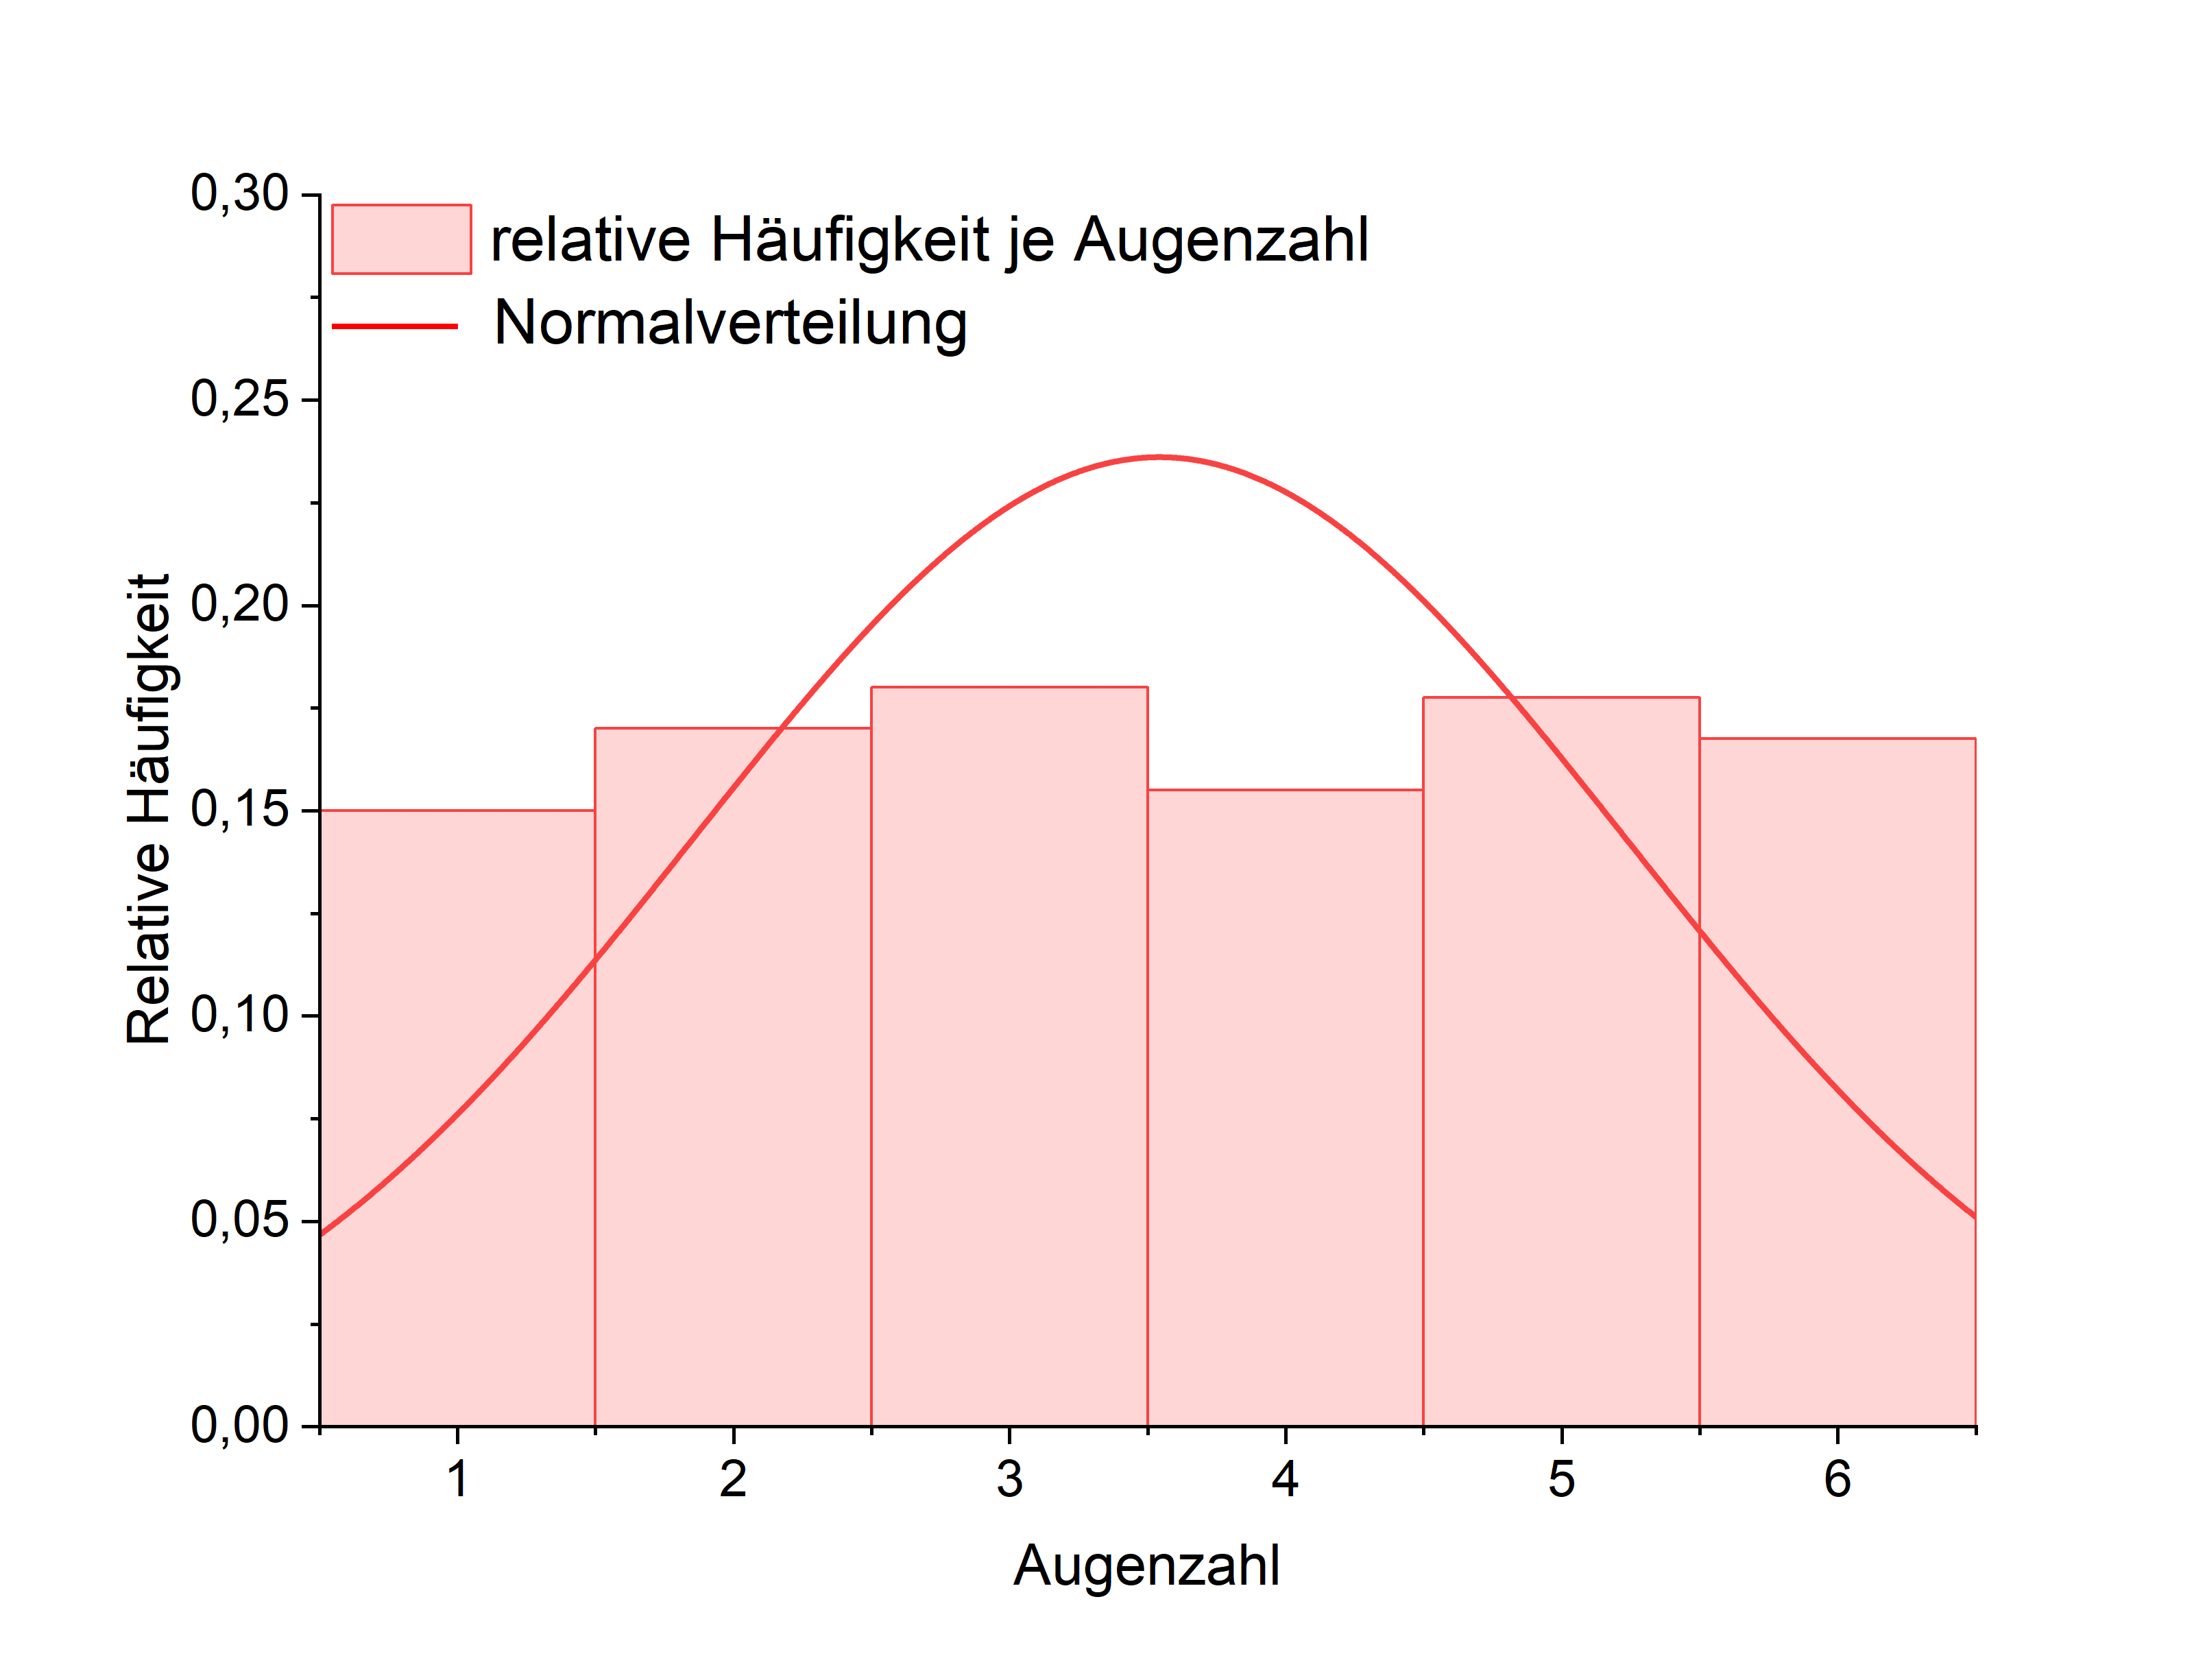
\includegraphics[width=\textwidth]{bilder/Diagramm1.png}        %// [ ] TODO: Diagramm Bild anpassen
    \caption{<>}                                                    %// [ ] TODO: Diagramm Bildunterschrift anpassen
\end{figure}

\section{Diskussion}
%//[ ] TODO: Diskussion
% Wie vergleicht sich meine Messung mit anderen Messungen/Theorien?
% Ist der Messwert sinnvoll? Stimmt die Größenordnung?
% Wo wurden Fehler gemacht? Was kann man verbessern?
% Gegebenenfalls rekursiv auswerten oder nachmessen!
% ursprüngliche Fragestellung diskutieren
% zB Standardabweichung diskutieren, berechnete Größen nennen

<>

\section{Anhang}
\label{sec:Anhang}

\end{document}
